\documentclass{article}
\usepackage[utf8]{inputenc}
\usepackage[main=russian,english]{babel}
\usepackage{caption}
\usepackage{subcaption}
\usepackage{graphicx}
\usepackage{hyperref}
\usepackage{geometry} % Простой способ задавать поля
\geometry{top=15mm}
\geometry{bottom=15mm}
\geometry{left=30mm}
\geometry{right=15mm}
\title{Lab work $5+$\\ Neural ODE }

\author{Safiullin Robert} 
\date{}
\begin{document}
\maketitle

\addtocontents{toc}{\setcounter{tocdepth}{-10}}


\subsection*{Motivation}
The motivation for this work was the desire to test how neural ODEs can be used to approximate the time series of solutions and phase portraits of a double pendulum.
\subsection*{Problem statement}
\begin{center}
    
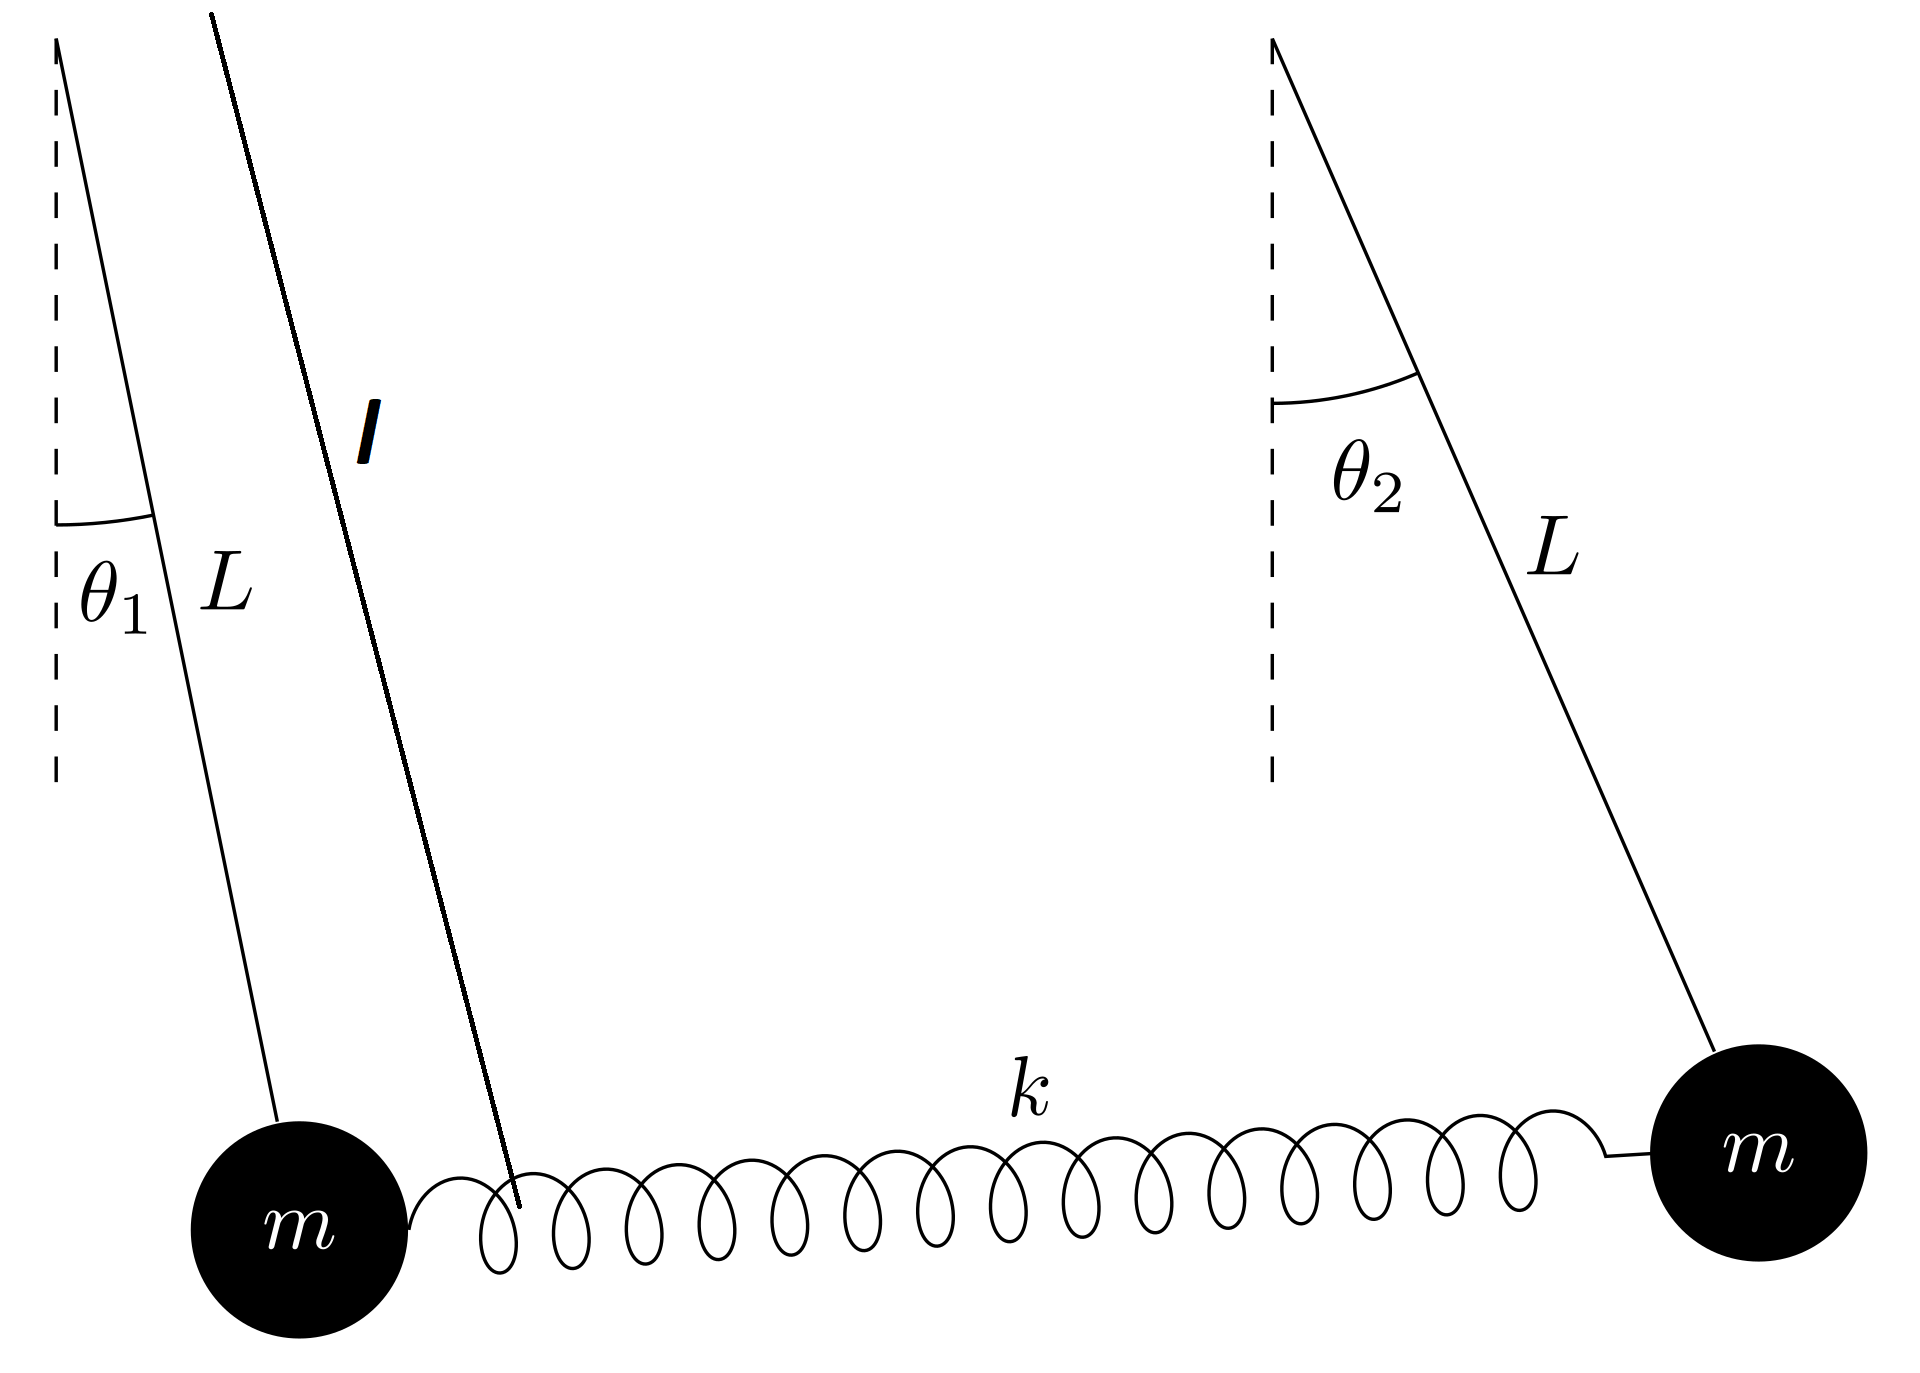
\includegraphics[scale = 0.1]{pendula.png}
\end{center}

A system consisting of two pendulums of length L, masses m, connected by a spring of length l is described by the following system of equations of motion: 
\begin{equation}
    m_1 L^2 \ddot{\theta_1} + m_1 g L \theta_1 = -kl^2(\theta_1 - \theta_2) 
\end{equation}
\begin{equation}
    m_2 L^2 \ddot{\theta_2} + m_2 g L \theta_2 = kl^2(\theta_1 - \theta_2)
\end{equation}
Initial conditions: \\
\begin{center}
    

$\theta_1(0) = 0$ \\
$\theta_2(0) = 0.44 \pi$ \\
$\dot{\theta_1}(0) = 0$ \\
$\dot{\theta_2}(0) = 0$ \\
L = l \\
$m_1 = m_2 = m$
\end{center}

\newpage

System solutions depending on time under the aforementioned conditions looks like this: \\
\begin{figure}[h]
     \centering
     \begin{subfigure}[b]{0.46\textwidth}
         \centering
         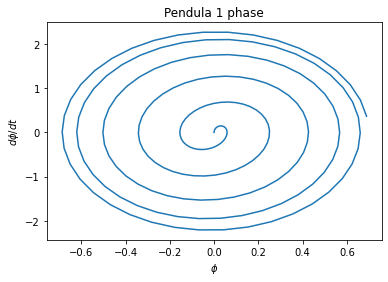
\includegraphics[width=\textwidth]{phase1.png}
         \caption{Pendula 1}
         \label{fig:y equals x}
     \end{subfigure}
     \hfill
     \begin{subfigure}[b]{0.46\textwidth}
         \centering
         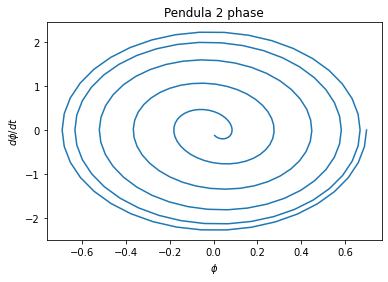
\includegraphics[width=\textwidth]{phase2.png}
         \caption{Pendula 2}
         \label{fig:three sin x}
     \end{subfigure}
     \hfill
     \begin{subfigure}[b]{0.45\textwidth}
         \centering
         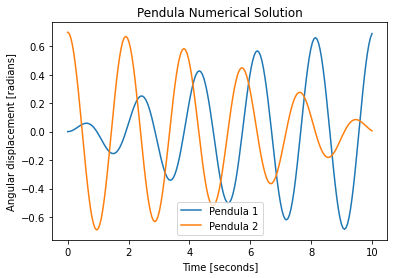
\includegraphics[width=\textwidth]{angle.png}
         \caption{Solutions}
         \label{fig:five over x}
     \end{subfigure}
        % \caption{Three simple graphs}
        \label{fig:three graphs}
\end{figure}


Plot and approximate its phase portrait  using ODE-net is required

\newpage

\subsection*{Problem solution}
\textbf{ODE - net}

Let there be a process obeying some unknown ODE and let several observations of its trajectory $(z_i, t_i), i \in [1..M]$ be known:
\begin{equation}
    \frac{dz}{dt} = f(z(t), t)
\end{equation}

It is required to approximate with a model the evolution of the system from the state ($z_0, t_0$) to the state ($z_1, t_1$). Let the function $\hat{f}(z, t, \theta)$ - be our model for approximating the dynamic function f(z,t). We need to choose a parameter $\theta$ so that our function coincides with the evolution of the system from the state $(z_0, t_0)$ for the time $t_1-t_0$ by dynamic function f(z,t). The loss function in this case will be written as follows: \\
\begin{equation}
    L(z(t_1) = L(\int^{t_1}_{t_0} f(z(t), t, \theta) dt) = L(ODESolve(z(t_0), f, t_0, t_1, \theta))
\end{equation}
The back propagation of the gradient of the ODE solution for sequential observations is calculated using the following algorithm: \\

\begin{figure}[h]
\centering
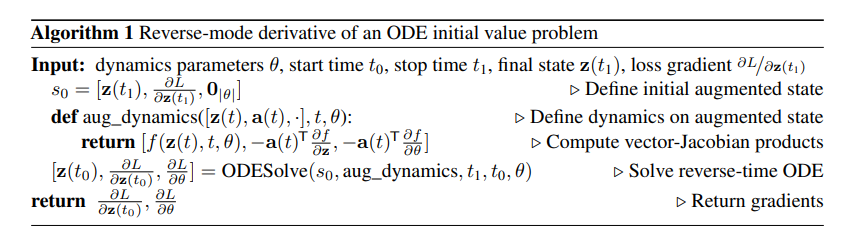
\includegraphics[scale = 0.75]{odenet.png}
\caption{Algorithm \protect\footnotemark}
\end{figure}

\footnotetext{Neural Ordinary Differential Equations, Ricky T. Q. Chen and Yulia Rubanova and Jesse Bettencourt and David Duvenaud,2019
      eprint=1806.07366
}


\newpage
\subsection*{Experiment}
We examine the influence of the choice of a numerical method for solving the ODE on the error in approximating the dynamics function $\mathbf{f(z,t)}$. To begin with, let's consider how the approximation $\mathbf{\hat{f}(z, t, \theta)}$ is constructed during optimization: \\
\begin{figure}[h]
     \centering
     \begin{subfigure}[b]{0.48\textwidth}
         \centering
         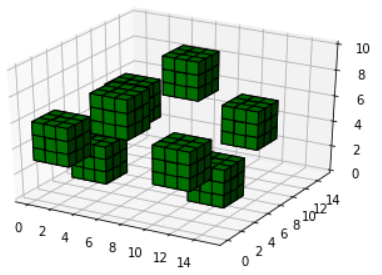
\includegraphics[width=\textwidth]{1.png}
        %  \caption{Pendula 1}
         \label{fig:y equals x}
     \end{subfigure}
     \hfill
     \begin{subfigure}[b]{0.48\textwidth}
         \centering
         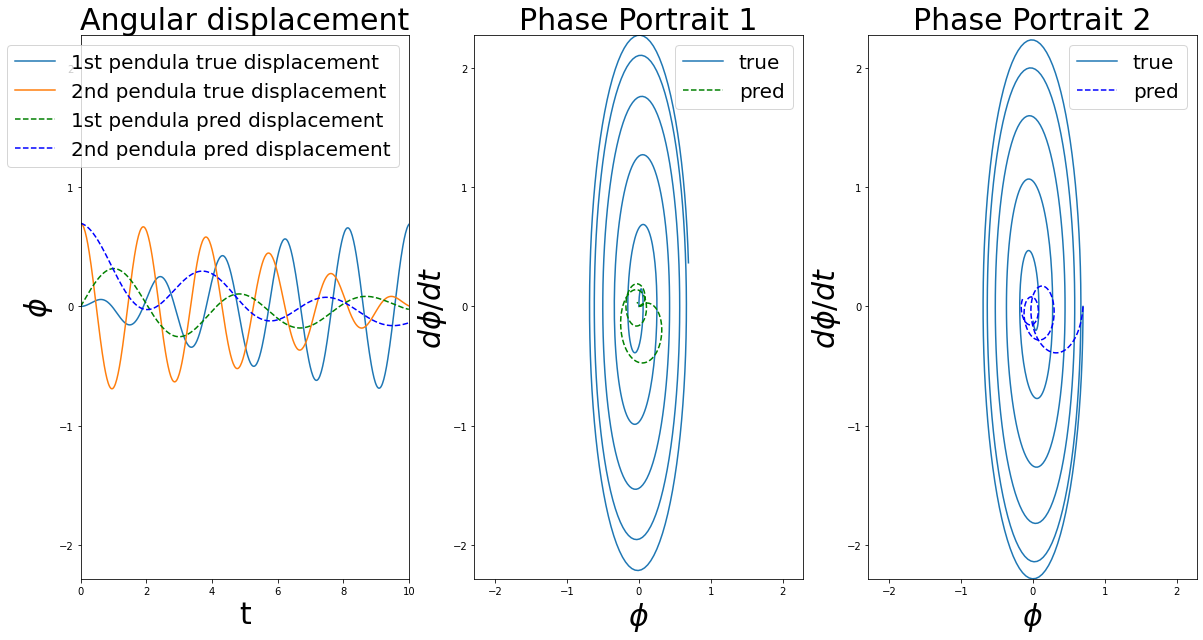
\includegraphics[width=\textwidth]{2.png}
        %  \caption{Pendula 2}
         \label{fig:three sin x}
     \end{subfigure}
     \hfill
     \begin{subfigure}[b]{0.48\textwidth}
         \centering
         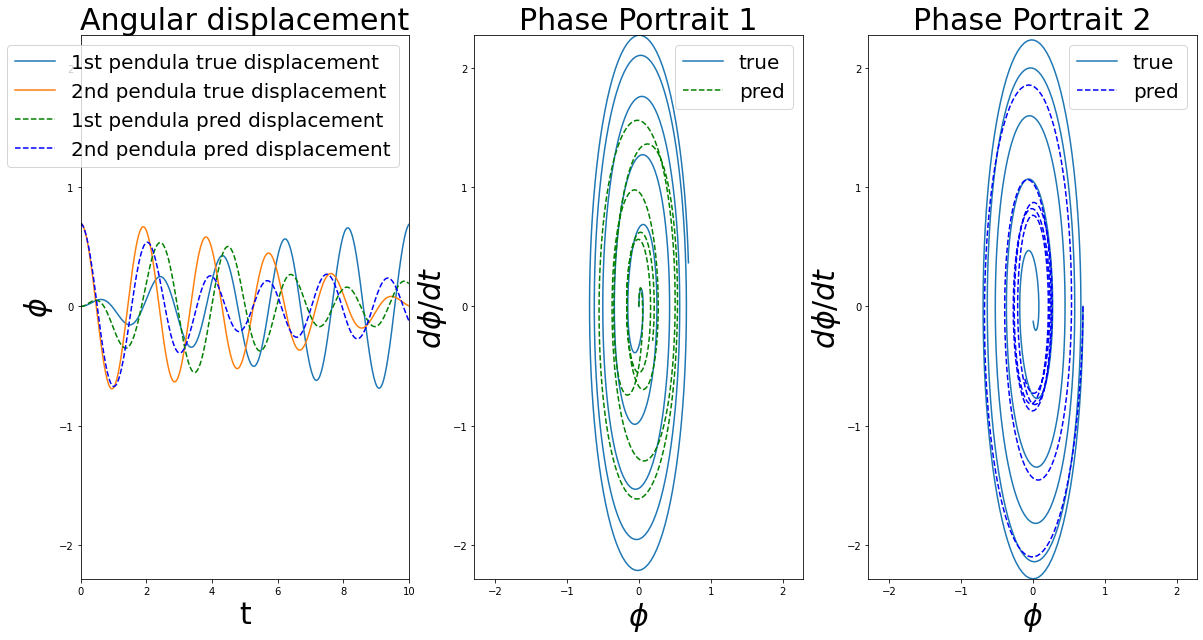
\includegraphics[width=\textwidth]{3.png}
        %  \caption{Solutions}
         \label{fig:five over x}
     \end{subfigure}
     \hfill
     \begin{subfigure}[b]{0.48\textwidth}
         \centering
         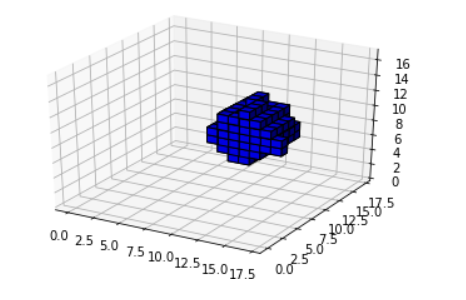
\includegraphics[width=\textwidth]{4.png}
         \caption{Solutions}
         \label{fig:five over x}
     \end{subfigure}
        \caption{Parameters tuning}
        \label{fig:three graphs}
\end{figure}

\begin{figure}[h]
    \centering
    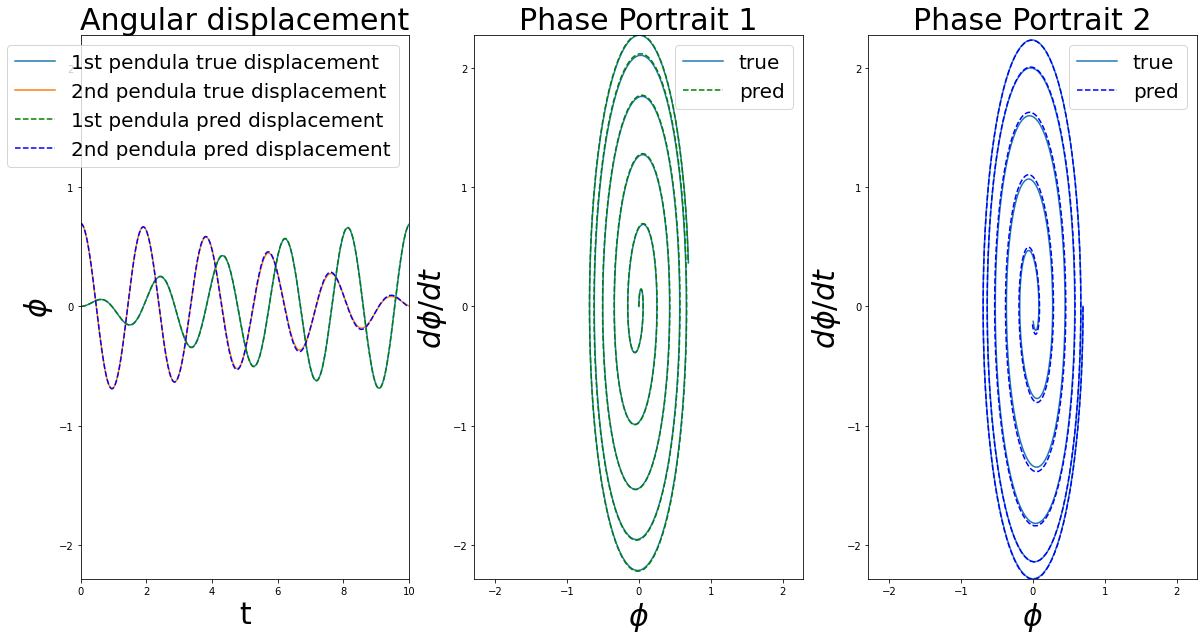
\includegraphics[scale = 0.3]{final.png}
\caption{Final approximation}
\end{figure}

\newpage
Next, we explore the influence of the selected numerical solutions on model quality using two methods with a fixed step and one with an adaptive one. Quantitatively, this process is presented in the following graph: \\
\begin{figure}[h]
\centering
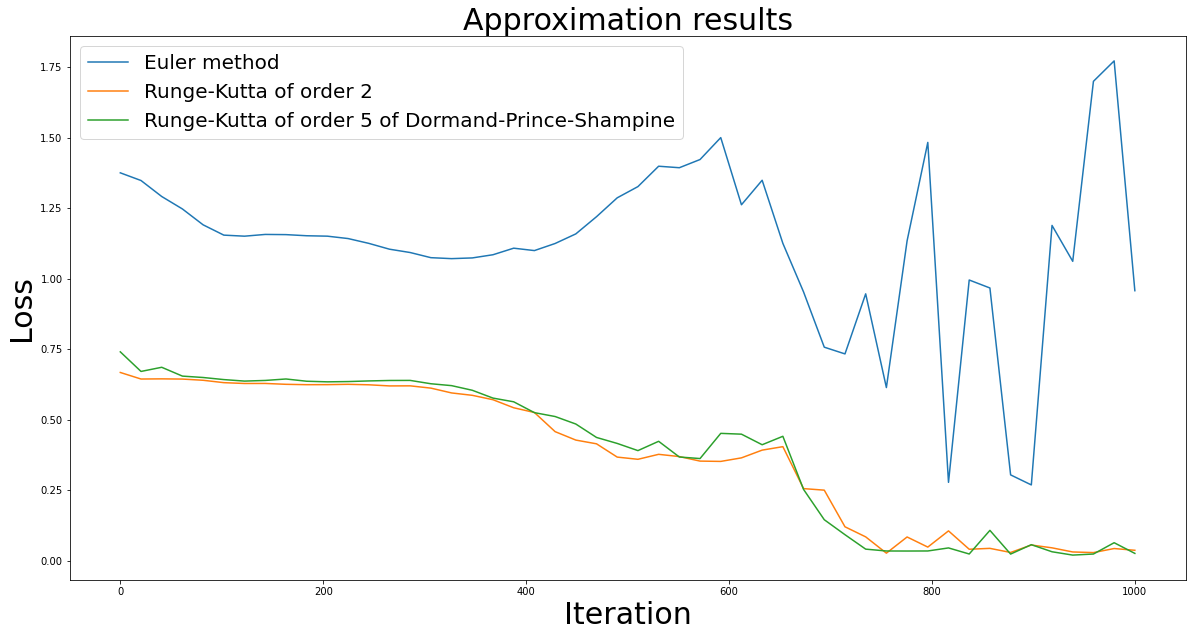
\includegraphics[scale = 0.35]{losses.png}
\caption{}
\end{figure} \\
As we can see, the simplest Euler method converges poorly to a function $\mathbf{f(z,t)}$ while more advanced higher-order approximation methods provide a good result (as in the above figure)


\newpage
\subsection*{Supplementary}
\href{https://arxiv.org/abs/1806.07366}{Neural Ordinary Differential Equations
} \\
\href{https://github.com/roberts2510/MMoF}{Github}\\
\href{https://en.wikipedia.org/wiki/Pendulum_(mechanics)#Coupled_pendula}{Data}

\end{document}